\chapter{Evaluation}
\label{chapter:evaluation}

The evaluation performed in the context of this thesis is threefold: First we present a case study, which demonstrates the major capabilities of the \textsc{Tavor framework} and how the framework can be applied to software programs using the example of a coin vending machine. Next we evaluate the generic fuzzing capabilities of \textsc{Tavor} by comparing it with \emph{aigfuzz}~\cite{2017_aig_fuzz}, a dedicated fuzzer for the \emph{AIGER} formats~\cite{biere2007aiger}. Finally we fuzz the JSON format and compare these generations with the manually written test suite of \textsc{Go}'s JSON package.

\section{Case Study: Coin Vending Machine}
\label{sec:evaluationCoinVendingMachine}

A \emph{coin vending machine} is the typical example for showcasing the practicality of model-based testing. In this section we introduce such a coin vending machine to give a step-by-step guide to the techniques presented in this thesis and to show how they can be applied to real world applications. The example is intentionally kept simple so that the basic functionality of each technique can be demonstrated. Source code that is not relevant for the demonstration but necessary for completeness can be found in \textsc{Tavor}'s \enquote{A Complete Example} documentation~\cite{2017_tavor-complete-example}.

The description of the demonstration is divided into the following subsections:

\begin{itemize}
\item Subsection~\ref{subsec:coinVendingMachineDefinition} defines our use-case of the coin vending machine and its implementation.
\item Subsection~\ref{subsec:coinVendingMachineKeywordDriven} defines the keyword-driven testing approach for defining test cases and to test the implementation.
\item Subsection~\ref{subsec:coinVendingMachineFormat} defines our test cases using the \textsc{Tavor Format}, and generates and executes a test suite using the \texttt{fuzz} command of \textsc{Tavor}.
\item Subsection~\ref{subsec:coinVendingMachineMutationTesting} executes the generated test suite and identifies missing test cases by applying code coverage metrics and \textsc{go-mutesting}.
\item Subsection~\ref{subsec:coinVendingMachineMutationDeltaDebugging} introduces some intentional bugs and reduces failing test cases that trigger these bugs using the \texttt{reduce} command of \textsc{Tavor}.
\end{itemize}

\subsection{Definition of the Coin Vending Machine}
\label{subsec:coinVendingMachineDefinition}

In this case study we consider a basic coin vending machine, which accepts coins of two different kinds: \texttt{coin25} and \texttt{coin50} representing credits of value 25 and 50. The coin vending machine keeps track of the currently accepted credit and vends if a credit of 100 is reached. One option to model this behavior, using a finite state machine, is shown in Figure~\ref{fig:coinVendingMachine}. Please note, that the given state machine could be defined more efficiently using state variables commonly used in model-based testing. While the \textsc{Tavor framework} supports such state variables, the \textsc{Tavor format} does not yet fully implement them. One possible direction of future work are such advancements of the \textsc{Tavor format}. Please refer to Chapter~\ref{sec:futureWork} for more details on proposed future extensions.

\begin{figure}[t]
\hspace*{-1.5cm}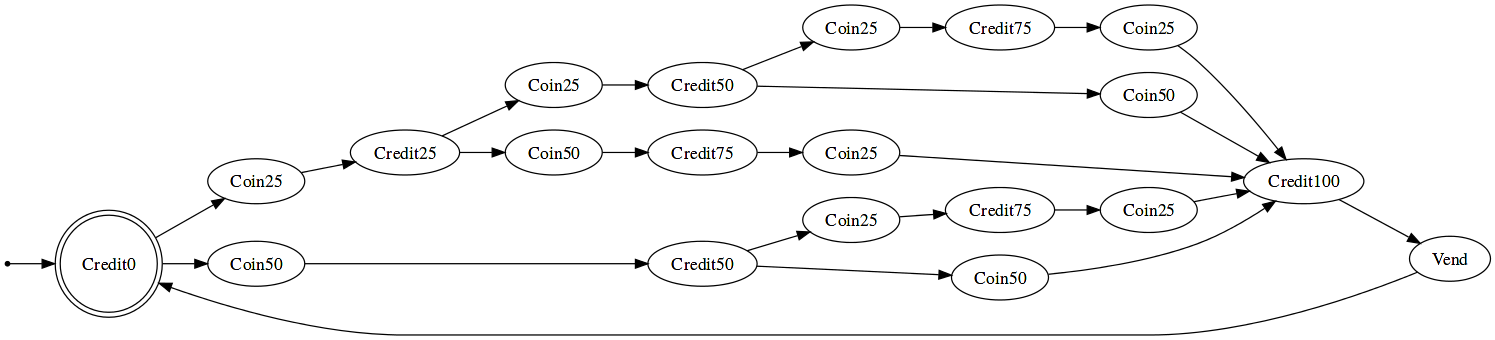
\includegraphics[width=1.1\textwidth]{images/evaluation-coin-vending.png}
\caption{Example Automaton of the Coin Vending Machine}
\label{fig:coinVendingMachine}
\end{figure}

In order to test the coin vending machine of our case study, an approach called keyword-driven testing is applied, which is explored in the next section.

\subsection{Keyword-Driven Testing}
\label{subsec:coinVendingMachineKeywordDriven}

The software testing technique \emph{keyword-driven testing}, introduced by Fewster et al.~in~\cite{fewster1999software}, also known as table-driven testing or action word based testing, separates the documentation of a test case from its implementation. Usually a sequence of keywords is used to specify the course of a test case, i.e., the sequence of keywords \texttt{Credit0, Coin50, Credit50, Coin50, Credit100, Vend, Credit0} specifies a sequence of actions to be executed for testing the coin vending machine. The implementation of the individual actions for each keyword, such as \texttt{Coin50}, is separated from the test case. Thus, making it possible to write test cases without any programming knowledge.

In order to apply keyword-driven testing a format needs to be defined, which specifies the structure of a keyword-driven test case. A test case can then be saved into a single file called a \emph{keyword-driven file}. Additionally, an executor is needed, which maps the individual keywords of such tests to concrete actions.

The \textsc{Tavor framework} offers the package \texttt{keydriven}, which provides various functionality to effectively apply keyword-driven testing. The function \texttt{ReadKeyDrivenFile} is used to parse a keyword-driven file and the type \texttt{Executor} is used to map keywords to their actions. Please consider Listing~\ref{lst:package-key-driven}, which outlines the most important types and functions of package \texttt{keydriven}. Next, we use this functionality to define an executor for the coin vending machine, whose interface is shown in Listing~\ref{lst:vending-machine-interface}. The interface of coin vending machine offers the functions \texttt{Credit}, \texttt{Coin} and \texttt{Vend}. For testing such a machine we introduce three keywords for our keyword-driven files with the following semantics: The keyword \texttt{credit} is used for validating the credit amount currently held by the vending machine, the keyword \texttt{coin} triggers the action of inserting a coin into the vending machine and finally the keyword \texttt{vend} invokes the vending action. Please note, that the keywords \texttt{coin} and \texttt{credit} need integer arguments specifying the coin credit amount.

\begin{listing}
\caption{Functionality of package \texttt{keydriven}}
\label{lst:package-key-driven}
\begin{gocode}
// ReadKeyDrivenFile reads in a keyword-driven file.
func ReadKeyDrivenFile(file string) ([]Command, error)

type Executor interface {
    // Register adds a given key-action pair to the executor.
    Register(key string, action Action) error
    // Execute executes a set of keyword-driven commands.
    Execute(cmds []Command)
}

// NewExecutor initializes and returns a new executor.
func NewExecutor() *Executor
\end{gocode}
\end{listing}

\begin{listing}
\caption{Interface of the Coin Vending Machine Module}
\label{lst:vending-machine-interface}
\begin{gocode}
type VendingMachine interface {
    // Credit returns the current credit of the coin vending machine.
    Credit() int
    // Coin inserts a coin into the coin vending machine and increases its credit.
    Coin(credit int) error
    // Vend executes a vend of the machine if enough credit (100) was put in and returns true.
    Vend() bool
}
\end{gocode}
\end{listing}

The executor connects the keyword-driven files, each representing a test scenario, with the implementation under test. It reads, parses and validates keyword-driven files, executes sequentially each key with its arguments by invoking actions of the implementation and validates these actions. A test passes if each action executes without any problems. The pseudocode for an executor for the coin vending machines of the case study is shown in Listing~\ref{lst:vending-machine-executor}. Please note, that the pseudocode does not include any error handling for the keyword-driven files and command line arguments in order to keep the code listing short. The main method subsequently parses the keyword-driven file, initializes the executor and executes the read commands. The actual connection between keywords and actions is made in function \texttt{initExecutor}, which registers for each keyword a callback function using the functionality of the provided package \texttt{keydriven}. Consider for instance the registration of the keyword \texttt{credit}, which includes one parameter denoting the expected amount of credit.\footnote{Validating the presence and type of keyword parameters has awas skipped to keep the pseudocode short.} When this keyword is encountered, the defined expected credit is compared with the currently held credit of the coin vending machine. In case these two values diverge, an error is returned, indicating that the test scenario failed.

\begin{listing}[hb]
\caption{Example Executor for a Coin Vending Machine}
\label{lst:vending-machine-executor}
\begin{gocode}
func main() {
  cmds := keydriven.ReadKeyDrivenFile(os.Args[1])
  executor := initExecutor()
  if err := executor.Execute(cmds); err != nil {
    os.Exit(exitFailed)
  }
  os.Exit(exitPassed)
}

func initExecutor() *keydriven.Executor {
  executor := keydriven.NewExecutor()
  machine := implementation.NewVendingMachine()
  executor.Register("credit", func(key string, parameters ...string) error {
    expected := strconv.Atoi(parameters[0])
    got := machine.Credit()
    if expected != got {
      return fmt.Errorf("Credit should be %d but was %d", expected, got)
    }
    return nil
  })
  executor.Register("coin", func(key string, parameters ...string) error {
    if err := machine.Coin(strconv.Atoi(parameters[0])); err != nil {
      return err
    }
    return nil
  })
  executor.Register("vend", func(key string, parameters ...string) error {
    if vend := machine.Vend(); !vend {
      return fmt.Errorf("Could not vend")
    }
    return nil
  })
  return executor
}
\end{gocode}
\end{listing}

The next step for testing the coin vending machine is to generate keyword-driven files, which is done in the next section by applying \textsc{Tavor's} format and fuzzing capabilities.

\begin{listing}
\caption{\textsc{Tavor Format} for Coin Vending Machine}
\label{lst:tavor-format-coin-vending}
\begin{gocode}
START = Credit0 *(Coin25 Credit25 | Coin50 Credit50)

Credit0  = "credit" "\t" 0 "\n"
Credit25 = "credit" "\t" 25 "\n" (Coin25 Credit50 | Coin50 Credit75)
Credit50 = "credit" "\t" 50 "\n" (Coin25 Credit75 | Coin50 Credit100)
Credit75 = "credit" "\t" 75 "\n" Coin25 Credit100
Credit100 = "credit" "\t" 100 "\n" Vend Credit0

Coin25 = "coin" "\t" 25 "\n"
Coin50 = "coin" "\t" 50 "\n"

Vend = "vend" "\n"
\end{gocode}
\end{listing}

\subsection{\textsc{Tavor Format} and Fuzzing}
\label{subsec:coinVendingMachineFormat}
 A valid keyword-driven file for the \textsc{Tavor framework}  needs to adhere to the following conditions: Each line starts with and holds at most one keyword. Each keyword may be followed by zero, one or more arguments, where each argument is preceded by a tab character. Finally each line ends with the new-line character. Combining the state machine shown in Figure~\ref{fig:coinVendingMachine}, the defined keys and the rules for the keyword-driven format together, results in the \textsc{Tavor format} shown in Listing~\ref{lst:tavor-format-coin-vending}.

This format file can now be easily fuzzed using the \textsc{Tavor} binary, resulting in outputs such as Listing~\ref{lst:key-driven-file-vending-machine}. Since there is a loop in the specified format, the graph can be traversed more than once, resulting in longer keyword-driven files which execute the action \texttt{vend} more than once. The default fuzzing strategy \texttt{Random} can create all possible permutations of a format but since it is random, it will need enough time to do so. Since even random events often lead to choosing the same path in a graph, many duplicated results will be generated using the \texttt{Random} fuzzing strategy. To work around this problem the \texttt{AllPermutations} strategy can be used which, as its name suggests, generates all possible permutations of a graph. This strategy should be used wisely since even small graphs can have an enormous amount of permutations. Also, since the example graph has a loop, we can state that there is an infinite amount of permutations. To work around this additional problem, the \texttt{---max-repeat} argument, which enforces a maximum for traversals and repetitions of loops, is used with a suitable value. Choosing a good value for \texttt{---max-repeat} is challenging, because high values may result in many repetitive permutations that will not improve the testing process. Choosing a small value on the other hand can lead to a bad coverage, which means that some scenarios are not tested.

\begin{listing}
\caption{Key-driven File for the Coin Vending Machine Test Scenario}
\label{lst:key-driven-file-vending-machine}
\begin{textcode}
credit  0
coin    25
credit  25
coin    50
credit  75
coin    25
credit  100
vend
credit  0
\end{textcode}
\end{listing}

The chosen \textsc{Tavor Format} for testing the coin vending machine of this case study is fairly easy to understand as it contains only a single loop. We choose the value $2$ for \texttt{\mbox{---max-repeat}} to ensure that the repetitive part of the state machine is executed at least once. By executing the following command: \texttt{tavor ---format-file vending.tavor ---max-repeat 2 fuzz ---strategy AllPermutations ---result-folder testset ---result-extension ".test"}. A total of 31 keyword-driven files is generated and stored in folder \texttt{testset}. Each written test file is named by \textsc{Tavor} according to its MD5 hash with the specified extension \texttt{.test}.

Since all components for testing the given state machine are now defined the next step is to execute the actual tests using the executor. One option to do this, is by invoking the program of Listing~\ref{lst:vending-machine-executor} for each test file, e.g., \texttt{go run executor.go testset/fba58bb35d28010b61c8004fadcb88a3.test}.

\afterpage{\clearpage}

Executing each keyword-driven file separately is tedious. A better solution would be to extend the executor, but this would also mean more restrictions and more flaw possibilities in the executor code. Alternatively a simple Bash script which executes each keyword-driven file of the folder \texttt{testset} and immediately exits if the execution of a file fails can be used. An example for such a Bash script is shown in Listing~\ref{lst:key-driven-test-script}.

\begin{listing}
\caption{Key-driven Test Script}
\label{lst:key-driven-test-script}
\begin{minted}[
  linenos,
  numbersep=5pt,
  breaklines,
  bgcolor=white,
]{bash}
#!/bin/bash
shopt -s nullglob
for file in testset/*.test
do
  echo "Test $file"
  ./executor $file
  if [ $? -ne 0 ]; then
    echo "Error detected, will exit loop"
    break
  fi
done
\end{minted}
\end{listing}

Executing this script reveals no errors, i.e., all tests passed. In the next section we introduce some defects into the implementation of the coin vending machine and check whether the test suite is able to reveal them.

\subsection{Mutation Testing}
\label{subsec:coinVendingMachineMutationTesting}

Although the test suite introduced in Subsection~\ref{subsec:coinVendingMachineFormat} passes, it is no guarantee that it verifies all functionality of the implementation of the coin vending machine. The first step to determine the quality of the test suite is to look at its code coverage. By converting the given test cases to ordinary \textsc{Go} test cases we can record their code coverage using the command\texttt{go test -coverprofile=coverage.out} followed by the command \texttt{go tool cover -html=coverage.out} to display the coverage information. Using this approach we determined that only three lines are not covered of an overall of 18 coverable lines. These three lines handle two negative cases of the coin vending machine: the first is the insertion of an unknown coin, i.e., an unknown coin amount, and the second is the invocation of the vending action, even though an amount of 100 credits has was reached. Both scenarios are not implemented in our model for generating test cases and are not implemented in the executor. Hence, new keywords would need to be introduced to generate and handle these scenarios. The shown code coverage and our interpretation of the results therefore match our model. However, code coverage only determines that a statement was executed but does not prove that a statement has actuawas verified.

The main purpose of mutation testing is to determine the quality of a test suite at hand by determining whether statements are tested by a given test suite. This technique, as well as \textsc{go-mutesting}, a framework for applying it, was introduced in detail in Chapter~\ref{chapter:goMutesting}. We apply mutation testing on our implementation and test suite by invoking the command \texttt{TESTSET=./testset/ go-mutesting coin}. Please note, that \enquote{./testset/} states the relative path to the directory holding the generated test cases and \enquote{coin} defines the \textsc{Go} package that should be analyzed. The relevant parts of the output for this command can be found in Listing~\ref{lst:mutation-testing-vending-machine} of Appendix~\ref{chapter:coinVendingMachine}. Since the implementation is rather simple, only a small amount of mutations can be applied. A total of five mutations were applied by \textsc{go-mutesting}, of whom three were killed by the generated test suite. This results in a mutation score of $3 / 5 = 0.6$. Investigating the two alive mutations shows the same result as with the code coverage analysis, i.e., only two negative cases are not covered. Hence, the used model to generate test cases applies to all possible positive test scenarios.

The remainder of this section discusses different flaws that can be introduced into the implementation of the coin vending machine, and checks, whether the previously generated test suite catches them. The following defects were introduced separately to the coin vending machine implementation:
\begin{enumerate}
\item \textbf{The \texttt{Coin} method no longer increases the credit:} This flaw can easily be introduced either by removing the addition in the \texttt{Coin} method, or by using a non-pointer type as receiver for the \texttt{Coin} method which leaves the state of the machine untouched.
\item \textbf{The \texttt{Vend} method no longer decreases the credit:} This flaw can be introduced along the same lines as the previous one, by either removing the subtraction in method \texttt{Credit} or by using a non-pointer type as a receiver.
\item \textbf{Every second 25 coin no longer increases the credit:} The defect type "works once but not twice" can be found in many programs. To emulate this kind of defect an additional state member was introduced to the coin vending machine implementation in order to trigger such a defect on every second call of method \texttt{Coin} with value 25.
\end{enumerate}

Please note, that the first two defect types are automatically introduced using \textsc{go-mutesting}. The third defect type on the other hand is not yet supported by the framework and needs to be introduced by hand.

The test suite from Section~\ref{subsec:coinVendingMachineFormat} was executed individually for each of the above flaws. Each defect type was successfully revealed, showcasing that the \textsc{Tavor framework} can be used to generate test suites with little effort, that are able to catch these implementation flaws. Besides its support for fuzzing and keyword-driven testing, the \textsc{Tavor framework} may be also used to apply delta-debugging in order to decrease debugging times. Applying delta-debugging to the coin vending machine case study is the content of the subsequent section.

\subsection{Delta-Debugging}
\label{subsec:coinVendingMachineMutationDeltaDebugging}

Delta-debugging, introduced in Section~\ref{sec:whatIsDeltaDebugging}, is a technique to automatically reduce error revealing inputs in order to make debugging easier for developers. Consider, for instance, a very long keyword-driven file revealing a defect. A developer would need to walk through a very long path through the state machine before she is able to find the cause of the problem. Often not the whole keyword-driven file is necessary to successfully reproduce the problem. When this is the case delta-debugging comes in handy to automatically reduce these keyword-driven files. The final result of the delta-debugging process should be a minimal test case, which still triggers the same defect as the original test case. This can be automatically or semi-automatically done by the \texttt{reduce} command of the \textsc{Tavor} binary. The binary uses our \textsc{Tavor format} file to parse and validate the given keyword-driven file and for reducing its data according to the rules defined by the format file. For instance optional content like repetitions can be reduced to a minimal repetition. In the coin vending machine case study the iterations of the vending loop can be reduced.

When executing test case \texttt{testset/fba58bb35d28010b61c8004fadcb88a3.test},\footnote{This test case was generation in Section~\ref{subsec:coinVendingMachineFormat}.} for the third defect type of Section~\ref{subsec:coinVendingMachineMutationTesting}, then the output in Listing~\ref{lst:key-driven-test-output} is generated. The introduced defect is triggered in the second vending iteration, because every second $25$ coin does not increase the machine's credit counter.

\begin{listing}
\caption{Key-driven Test Output}
\label{lst:key-driven-test-output}
\begin{textcode}
credit [0]
coin [50]
credit [50]
coin [50]
credit [100]
vend []
credit [0]
coin [50]
credit [50]
coin [25]
credit [75]
coin [25]
credit [100]
Error: Credit should be 100 but was 75
\end{textcode}
\end{listing}

First the semi-automatic method of the \textsc{Tavor} \texttt{reduce} command is applied to the test case at hand. The given format file is used to reduce the given input. Every reduction step displays the question "Do the constraints of the original input still hold for this generation?" to the user. The user's task is to inspect and validate the reduced output of the original data and decide by giving feedback if the defect is triggered (\texttt{yes}) or not (\texttt{no}). The following command starts this process: \texttt{tavor --format-file vending.tavor reduce --input-file testset/fba58bb35d28010b61c8004fadcb88a3.test}. Please refer to Listing~\ref{lst:semi-automated-delta-debug-vending-machine} of Appendix~\ref{chapter:coinVendingMachine} for the generated outputs of this command.

Semi-automatic processes can be tedious for big data especially due to the manual validation. The \textsc{Tavor} binary does therefore provide several methods to reduce the given inputs in a fully automated manner. The executor written in Section~\ref{subsec:coinVendingMachineKeywordDriven} was reused for this process. The reduction process is aided by the executor by exiting with different status codes on success or failure. The following command starts the fully automated delta-debugging process: \texttt{tavor --format-file vending.tavor reduce --input-file testset/fba58bb35d28010b61c8004fadcb88a3.test --exec "./executor TAVOR\_DD\_FILE" --exec-argument-type argument --exec-exact-exit-code}. Each exit status code of the executor is compared to the original exit status code. If it is not equal, the reduction process will try an alternative reduction step until a reduction path is found that which leads to the minimum. The output of the execution of this command is shown in Listing~\ref{lst:fully-automated-delta-debugging-output}.

\begin{listing}
\caption{Fully Automated Delta-Debugging for Coin Vending Machine}
\label{lst:fully-automated-delta-debugging-output}
\begin{textcode}
credit  0
coin    50
credit  50
coin    25
credit  75
coin    25
credit  100
vend
credit  0
\end{textcode}
\end{listing}

The fully automated delta-debugging step concludes our case study, which demonstrates the major capabilities of the \textsc{Tavor framework} and how they can be applied to facilitate model-based testing, fuzzing and delta-debugging on software programs.

\afterpage{\clearpage}

\section{Fuzzing the AIGER ASCII format}
\label{sec:evaluationFuzzingAigerAscii}

One of the major claims of the \textsc{Tavor framework} is to be a generic fuzzing tool, i.e., by providing the respective \textsc{Tavor format}, inputs of any format may be fuzzed. To evaluate this claim we compare the generations of \emph{aigfuzz}~\cite{2017_aig_fuzz}, a dedicated fuzzer for the AIGER formats~\cite{biere2007aiger}, with the generations of \textsc{Tavor}. In Subsection~\ref{subsec:evaluationIntroducingAigerAsciiFormat} we shortly introduce the AIGER ASCII format, subsequently Subsection~\ref{subsec:evaluationAigerExperimentalSetup} outlines the details of the experimental setup and finally Subsection~\ref{subsec:evaluationAigerResultsConclusions} presents the results and conclusions we draw from this evaluation.

\subsection{Introducing the AIGER ASCII format}
\label{subsec:evaluationIntroducingAigerAsciiFormat}

The AIGER ASCII format is used to model and-inverter graphs, containing inputs, outputs, latches, and-gates and inverters. We will discuss the structure and constraints of this format using its \textsc{Tavor format} definition shown in Listings~\ref{lst:tavor-aiger-ascii-format-1} and~\ref{lst:tavor-aiger-ascii-format-2}.\footnote{Please note, that the \textsc{Tavor format} definition was split up into two listings due to its length.}

\begin{listing}[H]
\caption{\textsc{Tavor format} denoting the AIGER ASCII format part one}
\label{lst:tavor-aiger-ascii-format-1}
\begin{minted}[
  mathescape,
  linenos,
  numbersep=5pt,
  breaklines,
  bgcolor=white,
]{go}
$Variable Sequence = start: 2,
                     step: 2
ExistingLiteral = 0, // false
                | 1, // true
                | $Variable.Existing,
                | ${Variable.Existing + 1} // +1 means a NOT for this input
Inputs = *(Input)
Input = $Variable.Next "\n"
Latches = *(Latch)
Latch = $Variable.Next " " ExistingLiteral "\n"
Outputs = *(Output)
Output = ExistingLiteral "\n"
ExistingLiteralAnd = 0, // false
                   | 1, // true
                   | ${Variable.Existing not in (AndCycle)},
                   | ${Variable.Existing not in (AndCycle) + 1} // +1 means a NOT for this input

// AndCycle finds all paths beginning from the variable andLiteral
AndCycle = ${andList.Reference path from (andLiteral) over (e.Item(0)) connect by (e.Item(2) / 2 * 2, e.Item(4) / 2 * 2) without (0, 1)}
Ands = *(And)
And = $Variable.Next<andLiteral> " " ExistingLiteralAnd " " ExistingLiteralAnd "\n"

Header = "aag ",
         (,                                                  // M
           ${Inputs.Count + Latches.Count + Ands.Count},
         | ${Inputs.Count + Latches.Count + Ands.Count + 1}, // M does not have to be exactly I + L + A there can be unused Literals
         ) " ",
         $Inputs.Count " ",                                  // I
         $Latches.Count " " ,                                // L
         $Outputs.Count " ",                                 // O
         $Ands.Count "\n"                                    // A
\end{minted}
\end{listing}

\begin{listing}
\caption{\textsc{Tavor format} denoting the AIGER ASCII format part two}
\label{lst:tavor-aiger-ascii-format-2}
\begin{minted}[
  mathescape,
  linenos,
  numbersep=5pt,
  breaklines,
  bgcolor=white,
]{go}
Body = Inputs,
       Latches,
       Outputs,
       Ands<andList>

Comments = "c\n",
           *(Comment)
Comment = *([\w ]) "\n"

Symbols = +0,$Inputs.Count(SymbolInput),
          +0,$Latches.Count(SymbolLatch),
          +0,$Outputs.Count(SymbolOutput)

SymbolInput = "i" $Inputs.Unique<=e> $e.Index " " +([\w ]) "\n"
SymbolLatch = "l" $Latches.Unique<=e> $e.Index " " +([\w ]) "\n"
SymbolOutput = "o" $Outputs.Unique<=e> $e.Index " " +([\w ]) "\n"

START = $Variable.Reset,
        Header,
        Body,
        ?(Symbols),
        ?(Comments)
\end{minted}
\end{listing}

Variables in the AIGER ASCII format are indexed using positive even integer values greater or equal to two, this coherence is modeled by using a sequence in the token \texttt{Variable}. Inverters in the AIGER ASCII format are denoted by setting the least significant bit of a literal, due to this reason only even integers are used for variables. Let us assume literal $2$ denotes an input to the and-inverter graph, then the literal $3$ is used to denote the negation of this input. All existing literals for the and-inverter graph are defined in token \texttt{ExistingLiteral}. The constants \texttt{TRUE} and \texttt{FALSE} are denoted using the literals $0$ and $1$. Additionally, all variables and their negations are part of all available existing literals.

The inputs and outputs of the and-inverter graph are represented by a single valid variable. A latch is defined by first listing its current state followed by its next state separated by a whitespace character. The AIGER ASCII format poses by far the most constraints on used and-gates. An and-gate is defined by first listing its left-hand side literal followed by its two right-hand side literals each separated by whitespace characters, e.g., for storing the result of the AND operation on the two variables 2 and 4 in variable 6 one would need to write \texttt{6 2 4}. This coherence is captured by token \texttt{And}. The AIGER ASCII format allows the connection of several and-gates, i.e., the left-hand side literal of an and-gate, or its negation, may be used in the right-hand side literal of another and-gate. However, it is prohibited to model cycles of and-gates in the and-inverter graph. Hence, the tokens \texttt{ExistingLiteralAnd} and \texttt{AndCycle} are necessary to ensure no cycles are generated by \textsc{Tavor}.

The header of the AIGER ASCII format starts with the string \texttt{aag} followed by five integers \texttt{M I L O A} separated by whitespace characters. Where \texttt{M} denotes the number of variables, \texttt{I} the number of inputs, \texttt{L} the number of latches, \texttt{O} the number of outputs and \texttt{A} the number of and-gates. The header is followed by the body of the format, listing consecutively the definitions of inputs, latches outputs and and-gates. The body is succeeded by an optional symbol table and an optional comment section. A symbol table is used to connect symbols, which are ASCII strings, to specific inputs, outputs or latches. Please note, that at most one symbol can be connected to a specific variable. In order to connect the first input with symbol \texttt{my\_input} we need to denote \texttt{i0 my\_input}. For more details on the constraints and structure of the AIGER ASCII format, please refer to~\cite{biere2007aiger}.

During the conduction of this evaluation we observed, that while it is possible to represent the AIGER ASCII format with the \textsc{Tavor framework}, it is a challenging task to come up with the correct format definition and semantics. Of course, it is still more time consuming to write a dedicated AIGER ASCII format fuzzer than defining its \textsc{Tavor format}, since a lot of boilerplate code and algorithms have to be created to handle the fuzzing part of the defined structures. Additionally, data structures as well as the architecture of such a dedicated fuzzer have to be defined and implemented instead of simply defining the syntax and semantics of a format, as can be done using the \textsc{Tavor format}. In the next subsections we will compare the generations of \textsc{Tavor} using the format defined in this subsection with the generations of the \emph{aigfuzz} fuzzer.

\subsection{Experimental Setup}
\label{subsec:evaluationAigerExperimentalSetup}

This subsection describes the experimental setup of this evaluation in detail. First we describe the hardware of the evaluation, then we outline how the test sets were generated and finally we describe the compilation and execution details.

\textbf{Hardware}\\
The generation of the test sets as well as their compilation and execution, have been executed in a KVM VM with OpenSUSE 42.3 as the hypervisor and guest operating system. The VM consisted of 4 virtual cores of an Intel Xeon CPU E3-1275 v5 with 3.60GHz, 16GB of DDR4 ECC RAM with a clock frequency of 2400 MHz and a dedicated volume to two Toshiba XG3 M.2 NVMe drives in a software RAID1 configuration.

\textbf{Test Set Generation}\\
In order to compare the generations of \emph{aigfuzz} with the generations of the \textsc{Tavor framework}, three different test sets were created. The first test set was generated using the command \texttt{aigfuzz -a}, in order to generate only AIGER ASCII format files using the aigfuzz tool. The remaining two test sets were created with the \textsc{Tavor framework} using the format introduced in Listings~\ref{lst:tavor-aiger-ascii-format-1} and~\ref{lst:tavor-aiger-ascii-format-2}. One is generated using the \emph{random} fuzzing strategy, where the parameter defining the maximum number of loop unrollings \texttt{max-repeat} is set to \texttt{10}, in order to ensure that also large files are being generated. The other test set is generated using the \emph{AlmostAllPermutations} fuzzing strategy, with \texttt{max-repeat} set to \texttt{1}\footnote{Higher values for \texttt{max-repeat} are currently not supported for the AIGER format in combination with the \emph{AlmostAllPermutations} fuzzing strategy due to an error in the generation of permutations.}.

For the randomly generated test sets a maximum of unique 10.000 test cases were generated. And for the \emph{AlmostAllPermutations} test set of \textsc{Tavor} all tests were created, i.e., 204 tests. Please note, that the number of possible tests for this fuzzing strategy is finite as it is bounded through the definition of \texttt{max-repeat}. Each of the generated test sets is stored in its own folder, where each generated file is stored named by its MD5 checksum using the file extension \texttt{.test}, e.g., \texttt{b6fe6a6049c39ab112f778769e92cc76.test}.

\textbf{Compilation and Execution}\\
The comparison of the three test sets is performed by measuring the code coverage they reach in the AIGER toolset, which provides various executables operating on AIGER ASCII files. For this experiment we used the AIGER toolset in version 1.9.4. from \url{http://fmv.jku.at/aiger/}.

In order to compile the toolset, we first created the default \texttt{Makefile} of the toolset by running \texttt{./configure}. Next this \texttt{Makefile} has been adapted to do compilations using Clang in version 4.0.1., by setting \texttt{CC=clang-4.0.1}. Additionally, we changed the environment variable \texttt{CFLAGS} to \texttt{-O3 -DNDEBUG -fprofile-instr-generate -fcoverage-mapping} to make the coverage information for each execution available, and the address sanitizer option \texttt{-fsanitize=address} was appended to \texttt{CFLAGS}, enabling the detection and reporting of memory errors during runtime. Finally we ran \texttt{make} to compile all binaries of the toolset with the defined configuration.

The LLVM developer tools were used to make the coverage information for this evaluation available. To run for instance the \texttt{aigand} tool on test case \texttt{12666cece4dbf5bfc1e1d46c02819da} of the \texttt{Random} fuzzing strategy the following command needs to be executed: \texttt{LLVM\_PROFILE\_FILE=./aiger/outa.profraw ./aiger/aigand ./aiger/tavor-random/12666cece4dbf5bfc1e1d46c02819da.test}. This command stores the coverage information of this execution in file \texttt{./aiger/outa.profraw}. Before this file can be used, it needs to be indexed using the following command \texttt{llvm-profdata merge -sparse outa.profraw -o outa.profdata}.

Figure~\ref{fig:code-coverage} depicts the relevant data which has been gathered for a single run. Code regions may span multiple lines, i.e., for blocks without any control flow. But it is also possible that a single line contains several regions, e.g., in \texttt{if(a || b)}. Lines inform about the lines of code that have been covered. Please refer to~\cite{2017_llvm_code_coverage}, for a detailed description of the used coverage tool and its workflows.

\begin{figure}[t]
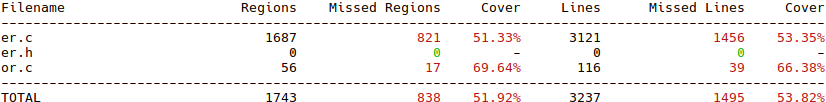
\includegraphics[width=\textwidth]{images/evaluation-code-coverage.png}
\caption{Code Coverage Example}
\label{fig:code-coverage}
\end{figure}

Since we run each test case separately per tool, we need to merge the code coverages for the individual runs in order to gain the cumulative coverage of a test set. To merge two code coverages the following command was executed: \texttt{llvm-profdata merge -sparse foo1.profraw foo2.profdata -o foo3.profdata}.

For automatically running each generated test on the tools of the AIGER toolset and computing their cumulative coverage per test set, a \textsc{Go} script has been devised. The pseudocode outlining the contents of this script is shown in Listing~\ref{lst:evaluation-script}. It iterates over the three test sets and cleans up their execution directory using the auxiliary function \texttt{cleanupExecutionDirectory}. For each of the AIGER tools used for this evaluation the tests of a test set are executed using the auxiliary function \texttt{execute}, which returns the coverage \texttt{c} as well as exit status \texttt{e} of the execution. These code coverages and exit states are stored and cumulated per tool and test set. Finally, the results of the evaluation are printed out for examination.

\begin{listing}
\caption{Pseudo Code for the Script for performing the AIGER Evaluation}
\label{lst:evaluation-script}
\begin{gocode}
testSets := [...]string{"aigFuzz -a", "tavarRandom", "tavorAllPerms"}
tools := [...]string{"aigand", "aigbmc -m", "aigflip", "aiginfo", ...}

for _, ts := range testSets {
  cleanupExecutionDirectory(ts)
  for _, tool := range tools {
    for _, t := range testsOfTestSet(ts) {
      c, e := execute(tool, t)

      cumulateCoverage(ts, tool, c)
      cumulateExitStatus(ts, tool, e)

      cleanup(t)
    }
  }
}

printResults()
\end{gocode}
\end{listing}

\subsection{Results and Conclusions}
\label{subsec:evaluationAigerResultsConclusions}

The statistic of the generated test sets is presented in Table~\ref{table:evaluationAIGERGeneration}, where column \texttt{Name} denotes the name of the test set using the naming convention <tool>-<fuzzing strategy>, \texttt{Cases} holds the number of unique tests in the test set, \texttt{Invalid} informs about the number of invalid generations, i.e., those not conforming to the format specification, \texttt{Size(MB)} holds the required disk space of the test set in megabytes and \texttt{Time(s)} informs about the time needed to generate the test set using the respective tool in seconds. When comparing the test set \texttt{aigfuzz-random} with \texttt{tavor-random} we observe that \textsc{Tavor}'s generation is almost twice as fast as the generation of \emph{aigfuzz}, which may be a result of the generated test set size. The tests generated by \emph{aigfuzz} are 3.5 times larger than the ones generated by \textsc{Tavor}. Additionally, \textsc{Tavor} generated 918 invalid tests which has not been done on purpose. Hence, either the format specification or the \textsc{Tavor framework} contains a bug. By far the smallest test set, with 204 tests, is represented by \texttt{tavor-aap}, which has been generated with the \emph{AlmostAllPermutations} fuzzing strategy.

\begin{table}
\caption{Comparison of the Test Set Generation of the AIGER Evaluation}
\label{table:evaluationAIGERGeneration}
\center
\begin{tabular}{| l | l | l | l | l |}
\hline \textbf{Name} & \textbf{Cases} & \textbf{Invalid} & \textbf{Size(MB)} & \textbf{Time(s)} \tabularnewline
\hline \emph{aigfuzz-random} & 10000 & 0 & 1125 & 143.90 \tabularnewline
\hline \emph{tavor-random} & 10000 & 918 & 40 & 82.70 \tabularnewline
\hline \emph{tavor-aap} & 204 & 0 & 0.8 & 1.40 \tabularnewline
\hline \end{tabular}
\end{table}

The 16 commands which were used for this evaluation are listed in Table~\ref{table:evaluationAIGERCommands}. On average these commands span 3400 lines of code and contain 1830 code regions per command.

\begin{table}
\caption{Comparison of the Commands of the AIGER Evaluation}
\label{table:evaluationAIGERCommands}
\center
\begin{tabular}{| l | l | l |}
\hline \textbf{Command} & \textbf{Lines} & \textbf{Regions} \tabularnewline
\hline \emph{aigand} & 3259 & 1749 \tabularnewline
\hline \emph{aigbmc} & 3477 & 1934 \tabularnewline
\hline \emph{aigflip} & 3264 & 1751 \tabularnewline
\hline \emph{aiginfo} & 3164 & 1704 \tabularnewline
\hline \emph{aigmiter} & 3332 & 1825 \tabularnewline
\hline \emph{aigmove} & 3272 & 1783 \tabularnewline
\hline \emph{aignm} & 3164 & 1704 \tabularnewline
\hline \emph{aigor} & 3237 & 1743 \tabularnewline
\hline \emph{aigsim} & 3832 & 2101 \tabularnewline
\hline \emph{aigsplit} & 3342 & 1768 \tabularnewline
\hline \emph{aigtoaig} & 3370 & 1794 \tabularnewline
\hline \emph{aigtoblif} & 3491 & 1887 \tabularnewline
\hline \emph{aigtocnf} & 3323 & 1799 \tabularnewline
\hline \emph{aigtodot} & 3348 & 1796 \tabularnewline
\hline \emph{aigtosmv} & 3388 & 1820 \tabularnewline
\hline \emph{aigunroll} & 4123 & 2167 \tabularnewline
\hline
\end{tabular}
\end{table}

The execution results of this experiment are shown in Table~\ref{table:evaluationAIGERExecution}. The \texttt{lines-missed} resp. \texttt{regions-missed} inform about source code lines resp. regions which have not been covered by the test set. Columns \texttt{lines-percentage} resp. \texttt{regions-percentage} inform about the covered lines resp. regions in percent. Next, the column \texttt{AddressSanitizer} denotes the number of executions for which LLVM's AddressSanitizer has been able to detect a problem. The number of runs for which an AIGER command exited with an exit status not equal to zero are captured in column \texttt{ExitStatusNotZero}. Finally, column \texttt{FileNotApplicable} denotes the number of test cases that have not been accepted, because their structure is not suitable for the respective command.

\begin{table}
\caption{Comparison of the Test Set Execution of the AIGER Evaluation}
\label{table:evaluationAIGERExecution}
\begin{small}
\begin{center}
\begin{threeparttable}
\begin{tabular}{| l | l | l | l | l | l | l | l | l | l | l | l |}
\hline
  \textbf{Command}
& \textbf{Test Set}
& \textbf{LM} % lines-missed
& \textbf{LP} % lines-percentage
& \textbf{RM} % regions-missed
& \textbf{RP} % regions-percentage
& \textbf{AS} %AddressSanitizer
& \textbf{ESNZ} % ExitStatusNotZero
& \textbf{FNA} % FileNotApplicable
\tabularnewline
\hline aigand & aigfuzz-random & 1822 & 44.09 & 972 & 44.43 & 0 & 0 & 0 \tabularnewline
\hline aigand & tavor-aap & 1682 & 48.39 & 908 & 48.08 & 0 & 0 & 0 \tabularnewline
\hline aigand & tavor-random & 1326 & 59.31 & 753 & 56.95 & 0 & 918 & 0 \tabularnewline
\hline aigbmc & aigfuzz-random & 2185 & 37.16 & 1243 & 35.73 & 0 & 0 & 0 \tabularnewline
\hline aigbmc & tavor-aap & 2096 & 39.72 & 1209 & 37.49 & 0 & 0 & 0 \tabularnewline
\hline aigbmc & tavor-random & 1716 & 50.65 & 1043 & 46.07 & 0 & 918 & 0 \tabularnewline
\hline aigflip & aigfuzz-random & 1857 & 43.11 & 994 & 43.23 & 0 & 0 & 0 \tabularnewline
\hline aigflip & tavor-aap & 3142 & 0.00 & 1692 & 0.00 & 99 & 99 & 0 \tabularnewline
\hline aigflip & tavor-random & 1367 & 58.12 & 780 & 55.45 & 4099 & 5017 & 0 \tabularnewline
\hline aiginfo & aigfuzz-random & 2104 & 33.50 & 1165 & 31.63 & 0 & 0 & 0 \tabularnewline
\hline aiginfo & tavor-aap & 2050 & 35.21 & 1148 & 32.63 & 0 & 0 & 0 \tabularnewline
\hline aiginfo & tavor-random & 1997 & 36.88 & 1114 & 34.62 & 0 & 918 & 0 \tabularnewline
\hline aigmiter & aigfuzz-random & 1552 & 53.42 & 880 & 51.78 & 0 & 0 & 0 \tabularnewline
\hline aigmiter & tavor-aap & 1580 & 52.58 & 891 & 51.18 & 0 & 10 & 10 \tabularnewline
\hline aigmiter & tavor-random & 1342 & 59.72 & 781 & 57.21 & 0 & 1763 & 845 \tabularnewline
\hline aigmove & aigfuzz-random & 1903 & 41.84 & 1024 & 42.57 & 0 & 0 & 0 \tabularnewline
\hline aigmove & tavor-aap & 1761 & 46.18 & 953 & 46.55 & 0 & 0 & 0 \tabularnewline
\hline aigmove & tavor-random & 1414 & 56.78 & 810 & 54.57 & 0 & 918 & 0 \tabularnewline
\hline aignm & aigfuzz-random & 2092 & 33.88 & 1158 & 32.04 & 0 & 0 & 0 \tabularnewline
\hline aignm & tavor-aap & 1996 & 36.92 & 1116 & 34.51 & 0 & 0 & 0 \tabularnewline
\hline aignm & tavor-random & 1985 & 37.26 & 1107 & 35.04 & 0 & 918 & 0 \tabularnewline
\hline aigor & aigfuzz-random & 1816 & 43.90 & 968 & 44.46 & 0 & 0 & 0 \tabularnewline
\hline aigor & tavor-aap & 1678 & 48.16 & 905 & 48.08 & 0 & 0 & 0 \tabularnewline
\hline aigor & tavor-random & 1322 & 59.16 & 749 & 57.03 & 0 & 918 & 0 \tabularnewline
\hline aigsim & aigfuzz-random & 2459 & 35.83 & 1404 & 33.17 & 0 & 0 & 0 \tabularnewline
\hline aigsim & tavor-aap & 2354 & 38.57 & 1359 & 35.32 & 0 & 0 & 0 \tabularnewline
\hline aigsim & tavor-random & 1980 & 48.33 & 1200 & 42.88 & 0 & 918 & 0 \tabularnewline
\hline aigsplit & aigfuzz-random & 1850 & 44.64 & 993 & 43.83 & 0 & 0 & 0 \tabularnewline
\hline aigsplit & tavor-aap & 1673 & 49.94 & 905 & 48.81 & 0 & 0 & 0 \tabularnewline
\hline aigsplit & tavor-random & 1360 & 59.31 & 779 & 55.94 & 0 & 918 & 0 \tabularnewline
\hline aigtoaig & aigfuzz-random & 2042 & 39.41 & 1078 & 39.91 & 0 & 0 & 0 \tabularnewline
\hline aigtoaig & tavor-aap & 1952 & 42.08 & 1030 & 42.59 & 0 & 0 & 0 \tabularnewline
\hline aigtoaig & tavor-random & 1588 & 52.88 & 879 & 51.00 & 0 & 918 & 0 \tabularnewline
\hline aigtoblif & aigfuzz-random & 2242 & 35.78 & 1268 & 32.80 & 0 & 0 & 0 \tabularnewline
\hline aigtoblif & tavor-aap & 2102 & 39.79 & 1194 & 36.72 & 0 & 0 & 0 \tabularnewline
\hline aigtoblif & tavor-random & 2050 & 41.28 & 1173 & 37.84 & 0 & 918 & 0 \tabularnewline
\hline aigtocnf & aigfuzz-random & 2326 & 30.00 & 1284 & 28.63 & 0 & 9967 & 9967 \tabularnewline
\hline aigtocnf & tavor-aap & 2257 & 32.08 & 1255 & 30.24 & 0 & 201 & 201 \tabularnewline
\hline aigtocnf & tavor-random & 2219 & 33.22 & 1233 & 31.46 & 0 & 9933 & 9015 \tabularnewline
\hline aigtodot & aigfuzz-random & 2229 & 33.42 & 1230 & 31.51 & 0 & 0 & 0 \tabularnewline
\hline aigtodot & tavor-aap & 2126 & 36.50 & 1192 & 33.63 & 0 & 0 & 0 \tabularnewline
\hline aigtodot & tavor-random & 2095 & 37.43 & 1168 & 34.97 & 0 & 918 & 0 \tabularnewline
\hline aigtosmv & aigfuzz-random & 2189 & 35.39 & 1222 & 32.86 & 0 & 0 & 0 \tabularnewline
\hline aigtosmv & tavor-aap & 2085 & 38.46 & 1176 & 35.38 & 0 & 0 & 0 \tabularnewline
\hline aigtosmv & tavor-random & 2063 & 39.11 & 1160 & 36.26 & 0 & 918 & 0 \tabularnewline
\hline aigunroll & aigfuzz-random & 3130 & 24.08 & 1648 & 23.95 & 0 & 9758 & 9758 \tabularnewline
\hline aigunroll & tavor-aap & 1593 & 61.36 & 912 & 57.91 & 0 & 10 & 10 \tabularnewline
\hline aigunroll & tavor-random & 3023 & 26.68 & 1597 & 26.30 & 0 & 9161 & 8243 \tabularnewline
\hline
\end{tabular}
\begin{tablenotes}
\textbf{LM}=lines-missed, \textbf{LP}=lines-percentage, \textbf{RM}=regions-missed, \textbf{RP}=regions-percentage, \textbf{AS}=AddressSanitizer, \textbf{ESNZ}=ExitStatusNotZero, \textbf{FNA}=FileNotApplicable
\end{tablenotes}
\end{threeparttable}
\end{center}
\end{small}
\end{table}

The experiment shows that \textsc{Tavor}'s \emph{random} fuzzing strategy reaches \texttt{2.6\% to 15.26\%} more coverage than \emph{aigfuzz}. Even though, \textsc{Tavor} generated substantially smaller files in less time. Since the coverage difference is considerable more than a few lines, the assumption that the invalid test cases generated by \textsc{Tavor} are solely responsible for the higher coverage can be neglected. Additionally, \textsc{Tavor}'s \emph{random} fuzzing strategy also led to more executions with exit states unequal to zero, which sometimes were due to the invalid test cases. For the commands \texttt{aigtocnf} and \texttt{aigunroll} there were cases which are valid but still led to non-zero exit states. Hence, \texttt{Tavor} did cover substantially more paths than \emph{aigfuzz}. Furthermore, a fault found by LLVM's AddressSanitizer was discovered during the execution of \textsc{Tavor}'s test suites for the command \texttt{aigflip} which \emph{aigfuzz} did not find.

In comparison \textsc{Tavor}'s \emph{AlmostAllPermutations} fuzzing strategy reached for 13 commands in average \texttt{3.32\%} more line coverage than \emph{aigfuzz}. For the command \texttt{aigunroll} a coverage of \texttt{61.38\%} was reached which even surpasses \textsc{Tavor}'s \emph{random} fuzzing strategy by \texttt{34.68\%}. However, the line coverage of the commands \texttt{aigflip} and \texttt{aigmiter} did not exceeded the coverage of \emph{aigfuzz}. Since these results have been generated with only \texttt{max-repeat} set to \texttt{1}, it can be assumed that a better coverage can be reached than with the \emph{random} fuzzing strategy when setting \texttt{max-repeat} to a higher value. However, the results for this test set are already astonishing since the coverage, surpassing \emph{aigfuzz} for 14 out of 16 commands, has been reached with substantially less test cases and generation time than with the other test sets.

All things considered, one explicit bug has been found in the AIGER toolset and continuous better line and regional coverage has been reached with \textsc{Tavor}'s \emph{random} fuzzing strategy in direct comparison to \emph{aigfuzz} a dedicated fuzzer for the AIGER format. Additionally, \textsc{Tavor}'s \emph{AlmostAllPermutations} fuzzing strategy reached better coverage for 14 out of 16 commands with its specific test case generation. Both fuzzing strategies reached these achievements with substantially smaller sized test cases and far less time for generating their test sets. In summary, this evaluation proved that \textsc{Tavor} as a generic fuzzer can keep up against a dedicated fuzzer, and that even a small amount of small-sized test cases can outperform a bigger test set.

\afterpage{\clearpage}

\section{Fuzzing the JSON Format}
\label{sec:evaluationJSON}

Handling sophisticated formats, such as the AIGER format presented in Section~\ref{sec:evaluationFuzzingAigerAscii}, is just one area where a generic fuzzer must excel. Another area are simple formats without any semantics but with lots of variety and recursive data structures. This section takes a look at the widely used JSON format, to evaluate that the \textsc{Tavor framework} can also efficiently define and fuzz such formats. The evaluation compares 3 generated test sets of \textsc{Tavor} with the manually written test suite of the JSON implementation \texttt{encoding/json} of the programming language \textsc{Go}. In Subsection~\ref{subsec:evaluationIntroducingJSONFormat} we shortly introduce the JSON format, subsequently Subsection~\ref{subsec:evaluationJSONExperimentalSetup} outlines the details of the experimental setup and finally Subsection~\ref{subsec:evaluationJSONResultsConclusions} presents the results and conclusions we draw from this evaluation.

\subsection{Introducing the JSON format}
\label{subsec:evaluationIntroducingJSONFormat}

The JSON (JavaScript Object Notation) format is a human-readable text format to depict JavaScript's data structures such as strings, numbers, arrays and name-value pairs. Even though JSON's name might suggest that it is bound to the programming language JavaScript, it is language-independent. Nowadays JSON is widely used for saving data and most commonly utilized for the communication between services. The format has been officially defined in RFC 7159\footnote{\url{https://tools.ietf.org/html/rfc7159}}. We will discuss the structure and constraints of this format using its \textsc{Tavor format} definition shown in Listing~\ref{lst:tavor-json-format}. Please note, that reading the RFC and defining this format took about 3 hours.

\begin{listing}[H]
\caption{\textsc{Tavor format} denoting the JSON format}
\label{lst:tavor-json-format}
\begin{minted}[
  mathescape,
  linenos,
  numbersep=5pt,
  breaklines,
  bgcolor=white,
]{go}
START = Value
Array = WS beginArray ?( Value *(valueSeparator Value) ) endArray WS
Object = WS beginObject ?( Member *(valueSeparator Member) ) endObject WS
Member = WS String WS nameSeparator Value // Member name, should be unique per object
Number = WS ?("-") (0 | [1-9]*([0-9])) ?("." +([0-9])) ?([eE] ?("-" | "+") +([0-9])) WS
String = WS "\"" *(Char) "\"" WS
Char = CharUnescaped | CharEscaped
CharUnescaped = [\x20-\x21] | [\x23-\x5B] | [\x5D-\x{10FFFF}] // 10FFFF -> 21bit of unicode
CharEscaped = "\\" (,
                     "\"", // quotation mark
                   | "\\", // reverse solidus
                   | "/", // solidus
                   | "b", // backspace
                   | "f", // form feed
                   | "n", // line feed
                   | "r", // carriage return
                   | "t", // tab
                   | "u" +4([a-fA-F0-9]), // 4 hex digits
                   )
Value = (,
          Object | Array  | Number | String,
        | WS "false" WS, // must be lower case
        | WS "null"  WS, // must be lower case
        | WS "true"  WS, // must be lower case
        )
// Helper
beginArray     = "["
beginObject    = "{"
endArray       = "]"
endObject      = "}"
nameSeparator  = ":"
valueSeparator = ","
WS = *([ \t\n\r])
\end{minted}
\end{listing}

The basic building block of the JSON format is a \texttt{Value} which represents every possible data structure of the format. A \texttt{Value} can be simple data such as a \texttt{Number} or a \texttt{String}, it can be a boolean value (\texttt{false}, \texttt{true}), the empty value \texttt{null} or it can contain combined values such as an \texttt{Array} or an \texttt{Object}, which defines name-value pairs. All of these definitions can be surrounded by whitespace characters. Even though, the value types \texttt{Number} and \texttt{String} store just simple data values, their representation can be rather complex, since they allow a variety of definitions, e.g., a \texttt{String} can consist of escaped and unescaped characters spanning the complete Unicode spectrum. For more details on the constraints and structure of the JSON format, please refer to RFC 7159.

During the conduction of this evaluation we observed that while \textsc{Tavor} is capable of fuzzing the format defined in Listing~\ref{lst:tavor-json-format}, it generates lots of test cases which look different to a human but exercise the same paths in a JSON implementation. To work around this problem, we defined a smaller format shown in Listing~\ref{lst:tavor-json-format-minimum}. The following reductions were made in comparison to the original format: first whitespace characters were completely removed from the generation, second the character generation was reduced to hold only the min and max permutations of the different character sets and lastly the number representation was reduced to a minimum set of interesting values. These manual reductions allowed to generate a smaller set of interesting test cases in a short amount of time. In the next subsections we will compare the generations of \textsc{Tavor} using the format defined in this subsection with the manually written test suite of the \texttt{encoding/json} package, the official implementation of the JSON format of the programming language \textsc{Go}.

\begin{listing}
\caption{\textsc{Tavor format} denoting a Minimum of the JSON format}
\label{lst:tavor-json-format-minimum}
\begin{minted}[
  mathescape,
  linenos,
  numbersep=5pt,
  breaklines,
  bgcolor=white,
]{go}
START = Value
Array = beginArray ?( Value *(valueSeparator Value) ) endArray
Object = beginObject ?( Member *(valueSeparator Member) ) endObject
Member = String nameSeparator Value
Number = "0" | "-0" | "949" | "999" | "-544" | "0.0" | "-0.0" | "0.4" | "0.00" | "0.40" | "-0.04" | "0e0" | "0e4" | "0E9" | "0e-9" | "0e+0" | "0e+9" | "0E-9" | "0E+0" | "0E+4" | "0e00" | "100E+99" | "140E+99" | "-999.99E+99"
String = "\"" *(Char) "\""
Char = CharUnescaped | CharEscaped
CharUnescaped = [\x20\x21\x23\x5B\x5D\x{10FFFF}]
CharEscaped = "\\" ( "\"" | "\\" | "/" | "b" | "f" | "n" | "r" | "t"  | "u" ("0000" | "FFFF") )
Value = Object | Array | Number | String | "false" | "null" | "true"
beginArray     = "["
beginObject    = "{"
endArray       = "]"
endObject      = "}"
nameSeparator  = ":"
valueSeparator = ","
\end{minted}
\end{listing}

\subsection{Experimental Setup}
\label{subsec:evaluationJSONExperimentalSetup}

This subsection describes the experimental setup of this evaluation in detail. First we outline how the test sets were generated and finally we describe the execution details. The hardware for the evaluation has the same setup as with the AIGER evaluation described in Subsection~\ref{subsec:evaluationAigerExperimentalSetup}.

\textbf{Test Set Generation}\\
In order to compare the manually written test suite of the JSON implementation \texttt{encoding/json} of the programming language \textsc{Go} with the generations of the \textsc{Tavor framework}, three different test sets were created. The fuzzing strategy \emph{AlmostAllPermutations} was used for all three test sets with \texttt{max-repeat} set to 1, 2 and 3 using the format introduced in Listing~\ref{lst:tavor-json-format-minimum}. Since this fuzzing strategy tries to generate targeted test cases and is bound to max-repeat, and finite set of test cases will be generated. Each of the generated test sets is stored in its own folder, where each generated file is stored named by its MD5 checksum using the file extension \texttt{.test}, e.g., \texttt{833f52bdb291f5915a6620fdaefe48bc.test}. Additionally to the three generated test set, we also included a combination of these three test sets and the manually written test suite as the fifth \enquote{combined} test set.

\textbf{Execution}\\
The comparison of the generated test sets to the manually written test suite of \texttt{encoding/json} is twofold. First we measure the code coverage they reach in the implementation of \texttt{encoding/json}, afterwards we perform mutation testing using \textsc{go-mutesting}, which was introduced in Chapter~\ref{chapter:goMutesting}. For this experiment we used \textsc{Go} in version 1.7.1 from \url{https://golang.org/dl/}.

Each generated test set is executed using its own \textsc{Go} test function, which loads all test cases and executes each of them separately using the function \texttt{testCase} of Listing\ref{lst:evaluationJSONTestFunction}. The test case function \texttt{testCase} calls only two functions of the \texttt{encoding/json} implementation, namely \texttt{Marshal} and \texttt{Unmarshal}, and checks their execution for errors. Therefore, it can be assumed that the generated test cases will cover far less of the implementation as the manually written test suite. Furthermore, since the generation only include valid cases, no error paths will be executed. Hence, a direct comparison of the code coverage is not appropriate. However, the results of the killed mutations during mutation testing can be directly compared, since they indicate tested paths in the implementation.

\begin{listing}
\caption{Test Function for Generated JSON Data}
\label{lst:evaluationJSONTestFunction}
\begin{gocode}
func testCase(t *testing.T, data []byte) {
  var o interface{}
  err := Unmarshal(data, &o)
  if err != nil {
    t.Fatal(err)
  }
  _, err = Marshal(o)
  if err != nil {
    t.Fatal(err)
  }
}
\end{gocode}
\end{listing}

Since all test sets as well as the manually written test suite are implemented using \textsc{Go} test functions, the execution of the evaluation can be done using \textsc{Go}'s testing tool and \textsc{go-mutesting}. The \texttt{encoding/json} implementation was copied in its own \texttt{GOPATH} environment and the test sets have been added to each execution. To execute a test set and measure its coverage the command \texttt{GOPATH=\$PWD/testset go test json -coverprofile=testset.coverage} was used, where \texttt{\$PWD/testset} indicates the folder to the given test set, \texttt{json} defines the package which should be tested and \texttt{testset.coverage} determines the coverage file for the test set. The execution of mutation testing was similarly performed using the command \texttt{GOPATH=\$PWD/testset go-mutesting json}.

\subsection{Results and Conclusions}
\label{subsec:evaluationJSONResultsConclusions}

The statistic of the generated test sets is presented in Table~\ref{table:evaluationJSONGeneration}, where column \texttt{Name} denotes the name of the test set, \texttt{Cases} holds the number of unique tests in the test set, \texttt{Size(MB)} denotes the required disk space of the test set in megabytes and \texttt{Time(s)} informs about the time needed to generate the test set in seconds. The \emph{max-repeat-1} includes no recursive data structures, while \emph{max-repeat-2} and \emph{max-repeat-3} include such structures and will therefore presumably reach more coverage. However, the later two test sets also include far more test cases and took more time to generate. Especially \emph{max-repeat-3} is a substantially larger test set and consumed a big amount of computational power for the generation of its test cases.

\begin{table}
\caption{Comparison of the Test Set Generation of the JSON Evaluation}
\label{table:evaluationJSONGeneration}
\center
\begin{tabular}{| l | l | l | l | l |}
\hline \textbf{Name} & \textbf{Cases} & \textbf{Size(MB)} & \textbf{Time(s)} \tabularnewline
\hline \emph{max-repeat-1} & 46 & 0.18 & 0.015 \tabularnewline
\hline \emph{max-repeat-2} & 1277 & 5.1 & 0.912 \tabularnewline
\hline \emph{max-repeat-3} & 71061 & 283 & 457.003 \tabularnewline
\hline \end{tabular}
\end{table}

The implementation of \texttt{encoding/json} consists of \texttt{1649} coverable statements, and \textsc{go-mutesting} found \texttt{1284} exercisable mutation of whom \texttt{147} are skipped because of various reasons, e.g., some mutations lead to uncompilable code. The execution results of this experiment are shown in Table~\ref{table:evaluationJSONResults}. The \texttt{Missed Statements} column informs about statements that are not covered by the test set. Next, the column \texttt{Statement Coverage in Percentage} detonates in percent how many statements have been covered. Finally, column \texttt{Killed Mutations} states how many mutations out of \texttt{1284} have been killed and are therefore checked by the test set.

\begin{table}
\caption{Comparison of the Test Set Results of the JSON Evaluation}
\label{table:evaluationJSONResults}
\center
\begin{threeparttable}
\begin{tabular}{| l | l | l | l |}
\hline \textbf{Name} & \textbf{MS} & \textbf{SCP} & \textbf{KM} \tabularnewline
\hline \emph{original} & 166 & 89.93 & 838 \tabularnewline
\hline \emph{max-repeat-1} & 1211 & 26.56 & 148 \tabularnewline
\hline \emph{max-repeat-2} & 1124 & 31.84 & 181 \tabularnewline
\hline \emph{max-repeat-3} & 1124 & 31.84 & 181 \tabularnewline
\hline \emph{combined} & 166 & 89.93 & 840 \tabularnewline
\hline
\end{tabular}
\begin{tablenotes}
\textbf{MS} = Missed Statements, \textbf{SCP} = Statement Coverage in Percentage, \textbf{KM}=Killed Mutations
\end{tablenotes}
\end{threeparttable}
\end{table}

The experiment shows that \textsc{Tavor}'s generated test sets reach \texttt{26.56\%} and \texttt{31.84\%} statement coverage solely by execution two functions of the underlying implementation, while the original manually written test suite covers \texttt{89.93\%}. Combining the original test suite with the generated test sets does not lead to any additional statement coverage. Both test set \emph{max-repeat-2} and \emph{max-repeat-3} have the same coverage and mutation testing result. Hence, the additional computational time for generating the third test set with \texttt{max-repeat} set to 3 did not accomplish any additional coverage for the JSON format. Looking at the mutation testing results reveals that the \emph{max-repeat-1} test set covered \texttt{11.52\%} and \emph{max-repeat-2} covered even \texttt{14.09\%} of the overall mutations. Surprisingly, combining the original test suite with the generated test sets resulted in \texttt{2} additionally killed mutations, i.e., two code paths that were not checked by the original test suite. Investigating this result reveals that these mutations are already killed by the \emph{max-repeat-1} test set. The first mutation shown in Listing~\ref{lst:killed-mutant-part-1} reveals that no test case of the original test suite checks upper-case characters in the third character of a Unicode escaped character, e.g., the escaped character \texttt{\textbackslash{}uAC3C} belongs to this class of characters since the character \enquote{3} is not an upper-case character. The second mutation shown in Listing~\ref{lst:killed-mutant-part-2} would be checked by parsing an empty JSON object \texttt{\{\}} into an object of an empty \textsc{Go} interface. These mutations manifest that a behavioral change for these two cases would not be caught by the existing test suite.

\begin{listing}[H]
\caption{Mutant Killed by Tavor Part One}
\label{lst:killed-mutant-part-1}
\begin{textcode}
--- /home/symflower/json/json/original/src/json/scanner.go  2017-12-01 18:53:42.663580118 +0100
+++ /tmp/go-mutesting-288106446//home/symflower/json/json/original/src/json/scanner.go.119  2017-12-03 10:43:45.026538957 +0100
@@ -378,7 +378,7 @@
 // stateInStringEscU12 is the state after reading `"\u12` during a quoted string.
 func stateInStringEscU12(s *scanner, c byte) int {
- if '0' <= c && c <= '9' || 'a' <= c && c <= 'f' || 'A' <= c && c <= 'F' {
+ if '0' <= c && c <= '9' || 'a' <= c && c <= 'f' || false {
    s.step = stateInStringEscU123
    return scanContinue
  }
FAIL "/tmp/go-mutesting-288106446//home/symflower/json/json/original/src/json/scanner.go.119" with checksum 3b91ecf37738b985eb6fa9a64bb9fcf9
\end{textcode}
\end{listing}

\begin{listing}[H]
\caption{Mutant Killed by Tavor Part Two}
\label{lst:killed-mutant-part-2}
\begin{textcode}
--- /home/symflower/json/json/original/src/json/decode.go 2017-12-01 18:53:43.147579808 +0100
+++ /tmp/go-mutesting-288106446//home/symflower/json/json/original/src/json/decode.go.183 2017-12-03 10:14:54.687623329 +0100
@@ -998,7 +998,7 @@
    op := d.scanWhile(scanSkipSpace)
    if op == scanEndObject {
      // closing } - can only happen on first iteration.
-     break
+
    }
    if op != scanBeginLiteral {
      d.error(errPhase)
FAIL "/tmp/go-mutesting-288106446//home/symflower/json/json/original/src/json/decode.go.183" with checksum 684f5c20122977ca389bb307ee0db6f7
\end{textcode}
\end{listing}


All things considered, no additional coverage but two additional killed mutations have been achieved by this quick evaluation of the JSON format and the official JSON implementation of the \textsc{Go} programming language. Additionally, one inconsistency has been cleaned up and one behavioral change has been made due to this evaluation\footnote{\url{https://codereview.appspot.com/162340043/}} in the \textsc{Go} project. These problems have been found, even though this implementation has been thoroughly tested since 2009. In summary, this evaluation proved that it is important to not solely rely on code coverage as a metric for stating the quality of a test suite but also to use more detailed analysis such as mutation testing. Additionally, we showed that \textsc{Tavor} fuzzing capabilities can be applied to diverse and highly recursive formats, and that its generations can lead with little effort to high coverage in a short amount of time.

\afterpage{\clearpage}
